%%%%%%%%%%%%%%%%%%%%%%%%%%%%%%%%%%%%%%%%%%%%%%%%%%%%%%%%%%
%
% Vzor pro sazbu kvalifikační práce
%
% Západočeská univerzita v Plzni
% Fakulta aplikovaných věd
% Katedra informatiky a výpočetní techniky
%
% Petr Lobaz, lobaz@kiv.zcu.cz, 2016/03/14
%
%%%%%%%%%%%%%%%%%%%%%%%%%%%%%%%%%%%%%%%%%%%%%%%%%%%%%%%%%%

% Možné jazyky práce: czech, english
% Možné typy práce: BP (bakalářská), DP (diplomová)
\documentclass[czech,BP]{thesiskiv}

% Definujte údaje pro vstupní strany
%
% Jméno a příjmení; kvůli textu prohlášení určete, 
% zda jde o mužské, nebo ženské jméno.
\author{Kateřina Kratochvílová}
\declarationfemale

%alternativa: 
%\declarationfemale

% Název práce
\title{Automatická anotace\\obrázků}

\thanktext{Ráda bych poděkovala Ing. Ladislavu Lencovi, Ph.D. za cenné rady, věcné připomínky, trpělivost a ochotu, kterou mi v průběhu zpracování této práce věnoval.}
% 
% Texty abstraktů (anglicky, česky)
%
\abstracttexten{The text of the abstract (in English). It contains the English translation of the thesis title and a short description of the thesis.}

\abstracttextcz{Bakalářská práce se zabývá automatickou anotací obrázků (AIA). Cílem práce je prověřit funkčnost vybraných metod z literatury a pokusit se o jejich vylepšení. Práce je zaměřena na metodu Joint Equal Contribution (JEC), kde bylo pozměněno přenášení klíčových slov. Dále byla vytvořena varianta rozšíření Patterns of Oriented Edge Magnitudes (POEM) na všechny barevné kanály. Metody jsou v teoretické části rozebrány a následně byly implementovány. V konečné fázy byly dosažené výsledky porovnány s literaturou. Testování probíhalo na datasetech iaprtc12 a ESP.
}

% Na titulní stranu a do textu prohlášení se automaticky vkládá 
% aktuální rok, resp. datum. Můžete je změnit:
%\titlepageyear{2016}
%\declarationdate{1. března 2016}

% Ve zvláštních případech je možné ovlivnit i ostatní texty:
%
%\university{Západočeská univerzita v Plzni}
%\faculty{Fakulta aplikovaných věd}
%\department{Katedra informatiky a výpočetní techniky}
%\subject{Bakalářská práce}
%\titlepagetown{Plzeň}
%\declarationtown{Plzni}

%%%%%%%%%%%%%%%%%%%%%%%%%%%%%%%%%%%%%%%%%%%%%%%%%%%%%%%%%%
%
% DODATEČNÉ BALÍČKY PRO SAZBU
% Jejich užívání či neužívání záleží na libovůli autora 
% práce
%
%%%%%%%%%%%%%%%%%%%%%%%%%%%%%%%%%%%%%%%%%%%%%%%%%%%%%%%%%%

% Zařadit literaturu do obsahu
\usepackage[nottoc,notlot,notlof]{tocbibind}

% Umožňuje vkládání obrázků
\usepackage[pdftex]{graphicx}

% import kvuli vkladani svg, import
\usepackage{graphicx, import}

% tabulky, viceradkove bunky 
\usepackage{multirow}

%barva u tabulek%
\usepackage[table]{xcolor}

%popisky u tabulek
\usepackage{caption}

%hezke cisla v textu%
\usepackage{siunitx}

%seznam u zkratek%
\usepackage{scrextend}

%vicesloupcova sazba%
\usepackage{multicol}

% Odkazy v PDF jsou aktivní; navíc se automaticky vkládá
% balíček 'url', který umožňuje např. dělení slov
% uvnitř URL
\usepackage[pdftex]{hyperref}
\hypersetup{colorlinks=true,
  unicode=true,
  linkcolor=black,
  citecolor=black,
  urlcolor=black,
  bookmarksopen=true}

% matematicke rovnice %
\usepackage{amsmath}

\usepackage{float}
% Při používání citačního stylu csplainnatkiv
% (odvozen z csplainnat, http://repo.or.cz/w/csplainnat.git)
% lze snadno modifikovat vzhled citací v textu
\usepackage[numbers,sort&compress]{natbib}

%%%%%%%%%%%%%%%%%%%%%%%%%%%%%%%%%%%%%%%%%%%%%%%%%%%%%%%%%%
%
% VLASTNÍ TEXT PRÁCE
%
%%%%%%%%%%%%%%%%%%%%%%%%%%%%%%%%%%%%%%%%%%%%%%%%%%%%%%%%%%
\begin{document}
%
\maketitle
\tableofcontents

\chapter{Úvod}

\par V dnešní době, kdy je svět přesycen obrázky v digitální podobě, není vůbec snadné nalézt obrázek zobrazující požadovaný obsah. Naneštěstí počítače nedokáží vnímat obraz jako lidé, vnímají totiž obrazy jako sérii binárních informací. Přitom počítače a jejich práce s obrazy by se dala využít v mnoha oborech jako je lékařství nebo doprava. Na základě toho vyplouvá na povrch problém jak spravovat digitální obrázky a efektivně mezi nimi vyhledávat. Prostřednictvím klíčových slov přiřazených k obrázkům se dá problém vyhledávání zjednodušit. Přiřazení klíčových slov probíhá pomocí procesu automatické anotace obrázků. Klíčová slova přiřazená k obrázku by měla vyjadřovat jeho obsah (například les, strom). Při reálném použití můžeme ovšem narazit na problém při zadávání abstraktních slov, například šťastná rodina.  

\par Pro automatickou anotaci obrázků se používá strojové učení. Můžeme ji rozdělit na dvě části. V první části získáme klíčové příznaky ve druhé už je samotná anotace, tedy přidělení klíčových slov. Abychom tento postup mohli provést v praxi, musíme nejdřív klasifikátor natrénovat pomocí trénovací množiny. Trénovací množina je množina obrázků, která již má ke každému obrázku přidána metadata s klíčovými slovy připravenými od lidí. Vybrané obrázky v trénovací množině by měly být různorodé, aby anotace probíhala správně. Pojem automatická anotace obrázků je jednoduše řečeno proces, při kterém jsou k obrázku automaticky přiřazena metada, která obsahují klíčová slova. 

\par Práce se bude zabývat nízkoúrovňovými příznaky konkrétně barvou a texturou. Ovšem v případě kdy požijeme barevný příznak ochudíme se o informaci o textuře obrázku, prozměnu když použijeme texturový příznak (který pracuje s šedotónovým obrázkem) zanedbáme informaci o barvě. Jako možnost zpřesnění klasifikátoru by se tedy dalo použít jejich zkombinování. Nabízí se několik řešení \cite{DiplomovaBrno}:   

\begin{description}
\item[Vyhodnotit a klasifikovat příznaky odděleně] 
a pak výslednou klasifikaci spojit z několika částí (například Joint Equal Contribution (JEC) \cite{JEC} ). Výhodou tohoto přístupu je zachování vlastností obou původních příznaků. Nevýhodou je náročnější výpočet a úspěšnost přístupu závisí na způsobu kombinace obou informací.

\item[Vytvoření společného příznaku] 
například rozšíření Patterns of Oriented Edge Magnitudes (POEM) na všechny barvené kanály. Musí se však dbát na to, že informace o barvě a textuře se mohou ovlinovat i protichůdně. 
\end{description} 

\par Cílem práce je navrhnout a implementovat software umožňující automatickou anotaci obrázků za použití nízkoúrovňových příznaků, konkrétně barvy a textury a jejich kombinací. Metody budeme zkoušet na standardních datech IAPRTC12 a ESP, následně výsledky porovnáme mezi sebou a s literaturou a pokusíme se o jejich vylepšení.

\chapter{JEC Joint Equal Contribution}
Tato metoda je založena na hypotéze, že podobné obrázky mají podobná klíčová slova. Pomocí metody hledání nejbližších sousedů (dále jen KNN) je nalezeno K nejpodobnějších obrázků. Přičemž klíčová slova od jednotlivých sousedů jsou posuzována odlišně a to právě na základě toho o kolik se s testovaným obrázkem liší. Metoda je postavena na dvou typech příznaků - barevných a texturových. 
\cite{JEC}

\section{Příznaky}
\par Barva a textura jsou považovány za dva nejdůležitější nízkoúrovňové příznaky pro obrázkovou reprezentaci. Nejběžnější barevné deskriptory jsou barevné histogramy, které jsou často využívány pro porovnávání a indexování obrázků, zejména z důvodu jejich efektivnosti a snadného výpočtu. K vytvoření texturových příznaků se používají Haarovy a Gaborovy wavelety a to především z důvodu, že jsou efektivní při vytváření řídkých a zároveň diskriminativných obrázkových rysů. Je-li žádoucí omezit vliv a předpoklady jednotlivých funkci a maximilizovat množství získaných informací, že využijeme několik jednoduchých a snadných výpočetních funkcí. 

\subsection{Barva}
\par U digitálního obrazu je barva reprezentovaná n-rozměrným vektorem. Jeho velikost a význam jednotlivých složek (tzv. barevných kanálů) zavisí na příslušném barevném prostoru. Počet bitů použitých k uložení buď celého vektoru nebo jeho jednotlivých složek se nazývá barevná hloubka (totožně bitová hloubka). Obvykle se můžeme setkat s hodnotami 8, 12, 14 a 16 bitů na kanál. 
\\
\par V použité metodě jsou získány vlastnosti z obrázků ve třech rozdílných barevných prostorech: RGB, HSV a LAB. RGB (Red, Green, Blue) je nejpoužívanější barevný prostor pro zachycení obrázu nebo jeho zobrazení. Oproti tomu HSV (Hue, Saturation and Value) se snaží zachytit barevný model tak jak ho vnímá lidské oko, ale zároveň se snaží zůstat jednoduchý na výpočet. Hue znamená odstín barvy (měří se jako poloha na standartním barevném kole $0^{\circ} - 360^{\circ}$ ), saturation je systost barvy (množství šedi v poměru k odstínu $0 \%$ šedá barva - $100 \%$ plně sytá barva) a value je hodnota jasu nebo také množství bílého světla (relativní světlost nebo tmavost barvy). Některé kombinace hodnot H, S a V mohou dávat nesmyslné výsledky. RGB je závislý na konkrétním zařízení, nemůže dosáhnout celého rozsahu barev, které vidí lidské oko, zatímco barevný model LAB je shopen obsáhnout celé viditelné spektrum a navíc je nezávislý na zařízení. L (ve zkratce LAB) značí Luminanci (jas dosahuje hodnot 0 - 100, kde 0 je černá a 100 je bílá). Zbylé A a B jsou dvě barvonosné složky, kdy A je ve směru červeno/zeleném a B se pohybuje ve směru modro/žlutém.

\begin{figure}[H]
		\centering
		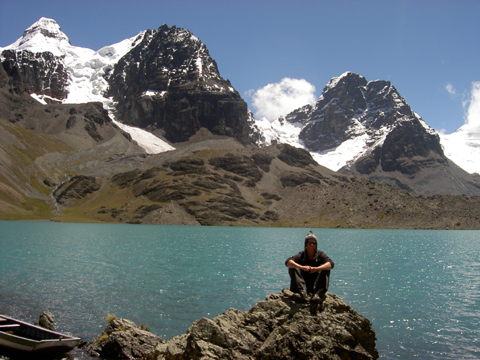
\includegraphics[height=100px]{./img/img_histogram.jpg}	
		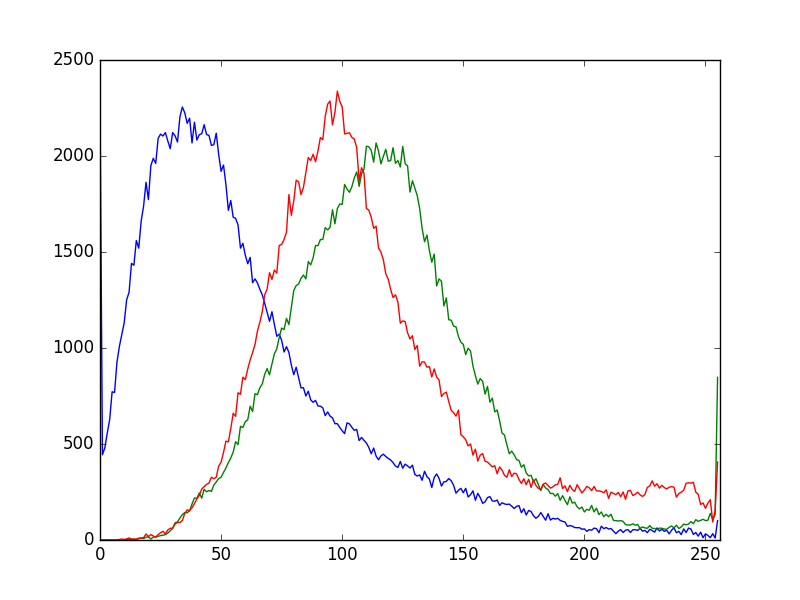
\includegraphics[height=100px]{./img/bgr_histogram.png}	
		\caption{RGB histogram - zastoupení jednotlivých složek v obrázku}
\end{figure}

\begin{figure}[H]
		\centering
		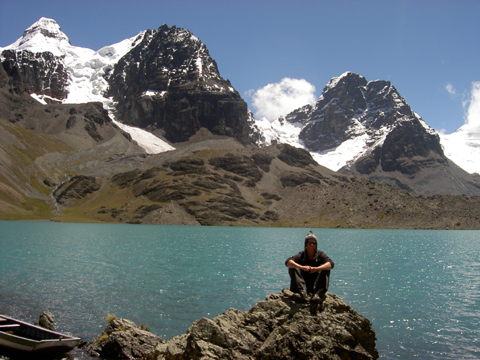
\includegraphics[height=100px]{./img/img_histogram.jpg}
		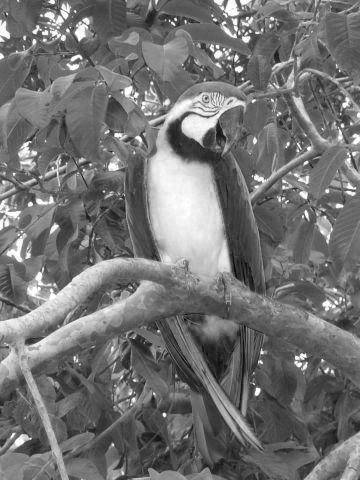
\includegraphics[height=100px]{./img/bgr_r.jpg}
		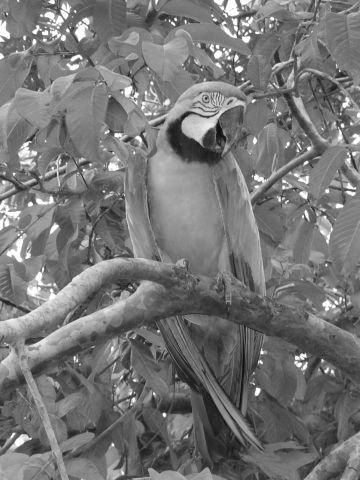
\includegraphics[height=100px]{./img/bgr_g.jpg}
		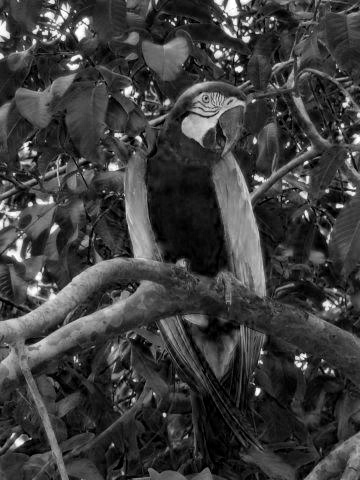
\includegraphics[height=100px]{./img/bgr_b.jpg}	
		\caption{Barevný prostor RGB a jeho jednotlivé složky v pořadí R, G, B}
\end{figure}

\begin{figure}[H]
		\centering
		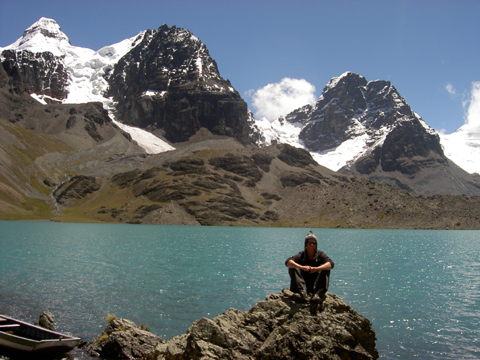
\includegraphics[height=100px]{./img/img_histogram.jpg}
		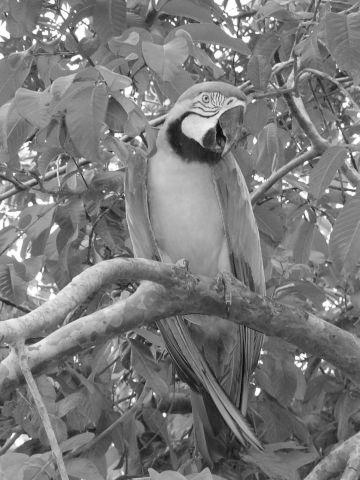
\includegraphics[height=100px]{./img/lab_l.jpg}
		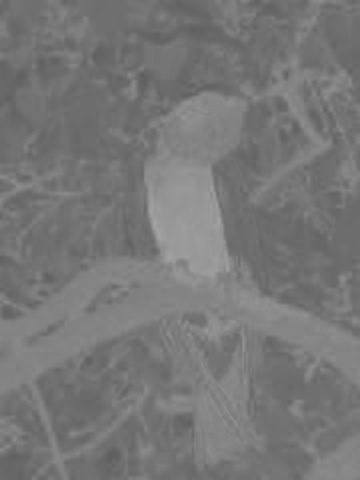
\includegraphics[height=100px]{./img/lab_a.jpg}
		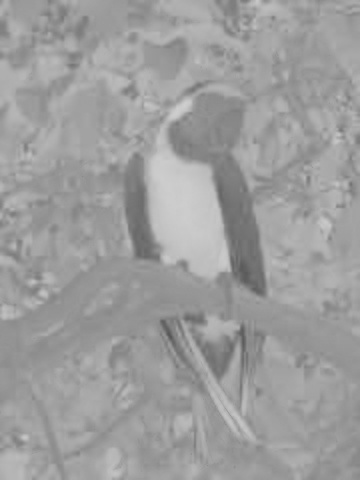
\includegraphics[height=100px]{./img/lab_b.jpg}	
		\caption{Barevný prostor LAB a jeho jednotlivé složky v pořadí L, A, B}
\end{figure}

\begin{figure}[H]
		\centering
		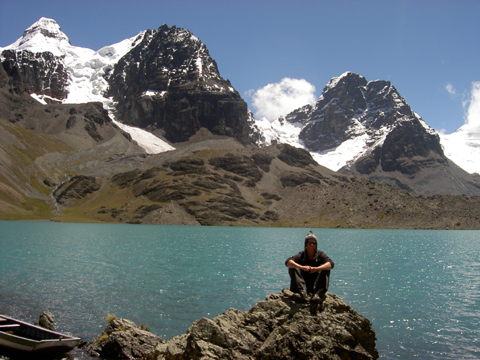
\includegraphics[height=100px]{./img/img_histogram.jpg}
		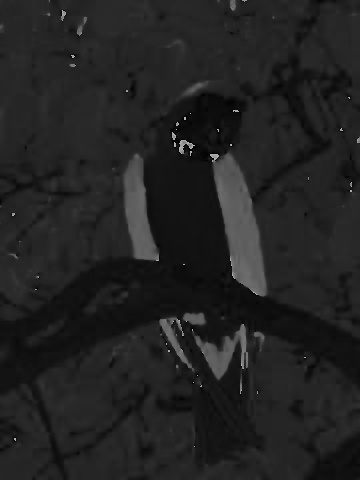
\includegraphics[height=100px]{./img/hsv_h.jpg}
		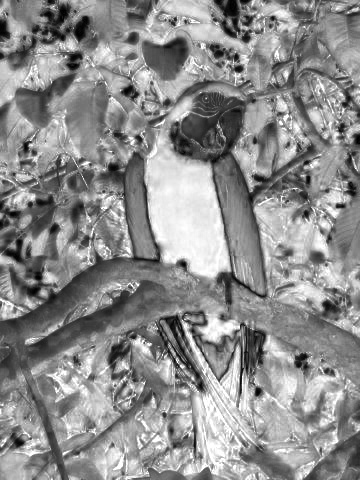
\includegraphics[height=100px]{./img/hsv_s.jpg}
		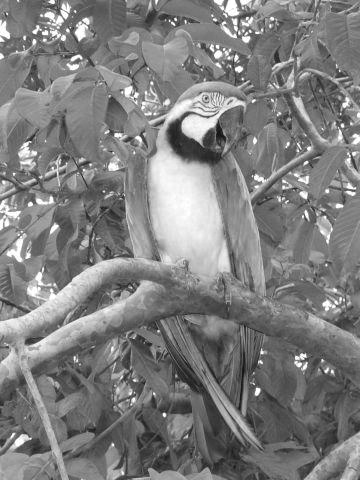
\includegraphics[height=100px]{./img/hsv_v.jpg}	
		\caption{Barevný prostor HSV a jeho jednotlivé složky v pořadí H, S, V}
\end{figure}

\par Pro RGB, HSV i LAB je použita barevná hloubka 16 bitů na kanál histogramu v jejich příslušném barevném prostoru. To znamená, že z každého barevného prostoru vzniknou tři šestnácti prvkové histogrami. Tyto histogrami jsou zřetězeny a následně použité jako reprezentace příslušného barevného prostoru.

\subsection{Textura}
\par Jako reprezentace textur a detekci hran budou použity Gaborovi a Haarovi vlnky (v originále Gabor a Haar wavelet). 

\subsubsection{Gabor}
\par Gaborův filtr je lineární filtr používaný pro analýzu textury, což znamená, že v podstatě zkoumá, zda existuje nějaký specifický frekvenční obsah v obraze ve specifických směrech v lokalizované oblasti kolem oblasti analýzy. Frekvence a orientace reprezentující Gaborovi filtry je podobná lidskému vnímání a proto je jejich použití zvláště vhodné při reprezentaci textury a detekci hran. V prostoru je 2D Gaborův filtr funkcí gausova jádra modulovaného sinusouvou rovinnou vlnou jak můžeme vidět v rovnici \ref{gabor_complex}.

\begin{figure}[H]
		\centering
		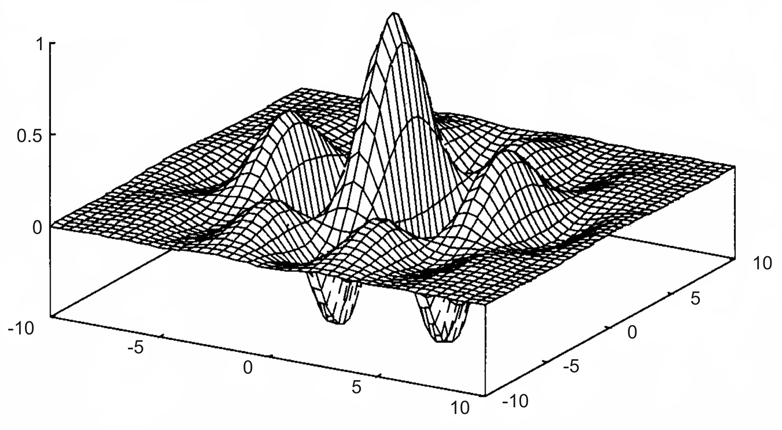
\includegraphics[height=200px]{./img/gabor.png}
		\caption{Gáborova vlnka je tvořena kombinací dvou cosinových funkcí, s rozdílnou frekvencí pro každou osu, a následně jsou vynásobeny dvourozměrnou Gaussovou funkcí \cite{Gabor}.} 					
\end{figure}

\begin{align}
   \label{gabor_complex}  g(x, y; \lambda, \theta, \psi, \sigma,  \gamma) = exp \Bigg( - \frac{{x^2 + \gamma^2 y^2}}{2 \sigma^2} \Bigg) exp \Bigg(i \bigg(2\pi \frac{x}{\lambda} + \psi \bigg)\Bigg)  
\end{align}

\par Gáborovi filtry jsou aplikovány na obrázky stejnou cestou jako běžné filtry. Základ tvoří maska (přesnější termín je konvoluční jádro), která reprezentuje filtr. Maskou je myšleno pole (obyvykle 2D protože se jedná o 2D obrázky) pixelů ve kterém každý pixel má přiřazenou hodnotu (váhu). Toto pole je přesunuto na každý pixel obrazu a je provedena konvoluční operace. Když je na obrázek aplikován gaborův filtr, poskytuje nejvyšší odezvu na hranach a místech, kde se textura mění. \cite{Gabor_wordpress}

\par Gaborův filtr reaguje na hrany a změny textury. Když se řekne, že filtr odpovídá na konkrétní funkci, myslí se tím že filtr má rozlišovací hodnotu v prostorové poloze této funkce (když se bude zabývat aplikací konolučních jader v prostoru - směru. Stejně platí i pro jinou oblast, jako frequence)

U Gaborova filtru máme několik parametrů, které ho ovlivňují. 
\paragraph{ksize} určuje velikost Gabor jádra. Když je ksize (a, b) je získáno jádro velikostí $a \times b$ pixelů. Jako u mnoha jiných konvolučních jader je preferován rozměr čtverce o lichých hranách (jen kvůli jednotnosti). Pří různých ksize se velikost konvolučního jádra mění. To také znamená, že konvoluční jádro je měřítko invariantní, protože zmenšení velikosti jádra je analogické k zmenšení velikosti obrazu. 

\paragraph{sigma} označuje standartní odchylka Gaussovi funkce použita v gaborově filtru. Tento parametr kontroluje šířku šířku Gausovi obalu použité v gabor jádře.

\paragraph{theta} je orientace normálu na paralelní pruhy Gaborovy funkce. Představuje možná jeden z nejdůležitějších parametrů gabor filtru. Theta rozhoduje jakého druhu funkce (na jaký typ funkce filtr reaguje). Například při nulév thetě bude filtr reagovat pouze na vodorovné příznaky. Proto abychom získali vlastnosti v různých úhlech obrazu, rozdělíme interval mezi 0-180 na několik stejných částí a vypočítáme Gaborovo jádro pro každou takto získanou hodnotu theta.

\paragraph{lambda} udává vlnovou délku sinusovky ve výše uvedené rovnici.

\paragraph{gamma} určuje prostorový poměr stran. Kontroluju elipsicitu gausovy funkce. Když je gamma = 1 je Gauss do kruhu (obalen kruhem)

\paragraph{psi} je fázový posun (určuje jestli nám vrátí reálnou nebo imaginární část). \\ 

\par Podle \citep{JEC} bude každý obrázek filtrován na třech vlnových délkách a čtyřech orientacích. Z každého z dvanácti obrázků bude histogram postaven skrze získané magnitudy. Vzniklé magnitudy zřetězíme a označíme jako příznak Gabor. Druhý příznak zachycuje Gabor faze. Příznak je označen jako GaborQ



\subsubsection{Haar}
\par Haarova vlnka je nejjednodušší vlnka, jejiž výhodou je především rychlý výpočet. Vlnka je realizována dvěma jednotkovými skoky, z čehož vzniknou dva obdelníkové pulzy s předchodem od kladného k zápornému. 

\begin{figure}[H]
    \centering
    %\def\svgwidth{\columnwidth}
    \def\svgwidth{200px}
    \import{img/}{haar_wavelet.pdf_tex} 
    \caption{Haarova vlnka. Převzato z \cite{HaarWiky}}
    %\input{soucet_vektoru.pdf_tex}
\end{figure} 

Předpis Haarovi vlnky: 
\begin{displaymath} 
	\label{haar} 
		    \psi(x) = \left\{ \begin{array}{r@{\quad}c}
    		1, & 0 \geq x \geq \frac{1}{2} \\
    		-1, & \frac{1}{2} \geq x \geq 1 \\ 
    		0, & jinde \\  \end{array} \right. 
\end{displaymath} 
\vspace{1cm}
 
\par Haarovi vlnové filtry reprezentují obrázek jako množinu oblastí a získavají průměrnou intenzitu z nejbližších sousedních oblastí. Jsou schopny extrahovat charakteristiky daných vlastností obrázku jako jsou například hrany nebo změny v textuře.  Při zpracovávání průměrné intenzity oblastí je snížena citlivost na šum a změny jasu. Velká množina haarovích filtrů se skládá z filtrů s různým počtem obdelníkových oblastí a s různými orientacemi vzhledem k vyzdvyžení různorodých texturových informací obrázku. Haarův vlnový filtr nabízí jednoduché a efektivní získávání informací z obrázků.
\par Základní Haarový vlnový filtr bere v potaz přilehlé obdelníkové oblasti v dané části obrázku a počítá rozdíl intenzit mezi nimi. 
 
\par Podle \citep{JEC} bude Haarova vlnka generovat konvoluční blok s Haarovými filtry na třech rozdílných orientacíh (horizontální, diagonální a veritkální). Použité na obrázky různých velikostí.  
% tohle se mi moc nelíbí chápu jak se to myslí ze to proste bude odpovídat(reagovat) na ty tři orientace 
 
\definecolor{ashgrey}{rgb}{0.7,0.75,0.71} 

\begin{multicols}{3}
	\begin{center}
		\begin{tabular}{ | c | c | }
    		\hline
    		\cellcolor{ashgrey!50}-1 & \cellcolor{ashgrey!50}-1 \\ \hline
    		1 & 1 \\ 
    		\hline
    	\end{tabular}
    	\vspace{0.5cm}
    	\par Vertikální
	\end{center}
	\begin{center}
		\begin{tabular}{ | c | c | }
    		\hline
    		\cellcolor{ashgrey!50}-1 & 1 \\ \hline
    		\cellcolor{ashgrey!50}-1 & 1 \\ 
    		\hline
    	\end{tabular}
		\vspace{0.5cm}
    	\par Horizontální
	\end{center} 	
	\begin{center}
		\begin{tabular}{ | c | c | }
    		\hline
    		\cellcolor{ashgrey!50}-1 & 1 \\ \hline
    		1 & \cellcolor{ashgrey!50}-1 \\ 
    		\hline
    	\end{tabular}
		\vspace{0.5cm}
    	\par Diagonální
	\end{center} 	
\end{multicols}

Výsledný příznak je možné vytvořit dvěma způsoby. První možností je výslednou matici, z každého velikosti i orientace, převést na 16 binový vektor. Tímto vyjde 12 šestnácti binových vektorů pro jeden obrázek, které jsou v konečné fázi zřetězeny. Dalsí možností je udělat z výsledné matice sumu, výsledným vektorem bude v tomto případě 12 prvkový vektor sum. 

\section{Vzdálenosti}
\par K určení příslušné vzdálenosti se můžeme setkat se čtyřmi měřítky vzdálenosti pro histogramy a rozdělení Kullaback-Leibler divergence KL - divergence, $\chi^2$ statistika, L1 - vzdálenost a L2 - vzdálenost. Na RGB a HSV je nejlépší použít L1 zatímco pro LAB je nejvhodnější KL - divergence. 

Problém s KL - divergencí nastává pouze tehdy, když se histogramy nebudou shodovat v nulách. Jeden předpoklad pro fungování tohoto vzorce je totiž že když je $Q(i) = 0$ tak zároveň musí být i $P(i) = 0$. \\

Kullaback-Leiber divergence:
\begin{align}
   \label{kl}  D_{KL} (P || Q) = \sum_{i} P(i) \log_e \bigg({\frac{P(i)}{Q(i)}} \bigg) 
\end{align}

L1 (jinak označováno jako Manhattan):
\begin{align}
   \label{L1} L_1 = \sum_{i=1}^{N} |x_i - y_i|  
\end{align}

L2 (jinak označováno jako Euklidovská vzdálenost)
\begin{align}
   \label{L2} L_2 = \sqrt{\sum_{i=1}^{N} (x_i - y_i)^2}  
\end{align}
 
\section{Kombinace vzdáleností}
Nejrozumnějším přístupem ke zkombinování vzdáleností od různých desktiptorů je aby jednotlivé vzdálenosti přispívali rovnoceně. Z tohoto důvodu je potřeba vzdálenosti přeškálovat na jednotné měřítko.\\
Označme si $I_i$ jako $i$-tý obrázek a řekněme, že máme $N$ jeho příznaků $f_i^1, ..., f_i^N$. Nadefinujme si $d_{(i,j)}^k$ jako vzdálenost mezi příznaky $f_i^k$ a $f_j^k$. Chtěli bychom zkombinovat všechny vzdálenosti příznaků mezi obrázky $I_i$ a $I_j$ tedy $d_{(i,j)}^k$ , $k=1, ..., N$.  Vzdálenosti nám ale v praxi nevyjdou tak aby měli stejný poměr na výsledku, proto předtím než vzdálenosti zkombinujeme musíme je normalizovat do jednotné formy. Získáme maximální a minimální hodnotu pro každý příznak a na základě toho hodnotu přeškálujeme na interval od 0 do 1. Jestliže označíme přeškálovánou vzdálenost jako ${\tilde{d}_{(i,j)}^k}$ následně můžeme označit kompletní vzdálenost mezi obrázky $I_i$ a $I_j$ jako \eqref{jec} Joint Equal Contribution (JEC). 


\begin{align}
   \label{jec} JEC = \sum_{k=1}^N\frac{\tilde{d}_{(i,j)}^k}{N}
\end{align}

\section{Přenesení klíčových slov}
Pro přenesení klíčových slov je použita metoda, kdy je přeneseno $n$ klíčových slov k dotazovanému obrázku $\tilde{I}$ od K nejbližších sousedů z trénovací sady. Je nadefinováno $I_{i}, i = 1, ..., K$ ,těchto K nejbližší sousedů je seřazeno podle vzrůstající vzdálenosti (tzn. že $I_{1} $ je nejvíce podobný obrázek). Počet klíčových slov k danému $I_{i}$ je označen jako $|I_{i}|$. Dále jsou popsány jednotlivé kroky alogoritmu na přenesení klíčových slov.
\begin{enumerate}
	\item Klíčová slova z $I_{1}$ jsou seřazeno podle jejich frekvence výskytu v trénovací sadě.
	\item Ze všech $|I_{1}|$ klíčových slov z $I_{1}$ je přeneseno $n$ nejvýše umístěná klíčová slova do dotazovaného $\tilde{I}$. Když $|I_{1}| < n$ algoritmus pokračuje na krok 3. 
	\item Klíčová slova sousedů od $I_{2}$ do $I_{K}$ jsou seřazena podle dvou faktorů
	\begin{enumerate}
		\item výskytu v trénovací sadě s klíčovými slovy přenesených v kroku 2
		\item místní frekvence (tj. jak často se vyskytují jako klíčová slova u obrázků $I_{2}$ až $I_{K}$). Jsou vybrána nejvíce vyskytující $n-|I_{1}|$ klíčových slov převedených do $\tilde{I}$.
	\end{enumerate}
\end{enumerate}

Tento algoritmus pro přenos klíčových slov je poněkud odlišný od algoritmů, které se běžně používají. Jeden z běžně užívaných funguje na principu, že klíčová slova jsou vybrána od všech sousedů (se všemi sousedy je zacházeno stejně bez ohledu na to jak jsou danému obrázku podobní), jiný užívaný algoritmus k sousedům přistupuje váženě (každý soused má jinou váhu)a to na základě jejich vzdálenosti od testovaného obrázku. Při testování se ovšem ukázalo, že tyto přímé přístupy přináší horší výsledky v porovnání s použitým dvoufaktorovým algoritmem pro přenos klíčových slov. \\
V souhrnu použitá metoda je složenina ze dvou složenin a to obrázkové vzdálenosti (JEC) a výše popsaným algoritmem na přenášení klíčových slov. 
 
\chapter{POEM}
POEM (Patterns of Oriented Edge Magnitudes). Vstupem algoritmu se předpokládá šedotónový obrázek o rozměrech  $m \times n$. Jelikož většinou je vložený barevný obrázek, musí být po načtení převeden na šedotónový. \cite{SrovnaniDeskriptoru}

\subsection{Výpočet gradientu a magnitudy}
Nejprve je potřeba vypočítat gradient. Gradient je obecně směr růstu. Výpočet může probíhat různými způsoby. Jednou z možností je použít masku, kterou aplikujeme na vstupní obrázek. Podle některých studii jsou nejlepší jednoduché masky jako je např. $[1, 0, -1]$ a $[1, 0, -1]^{\,t}$. Okraje obrázku se buď vypouštějí nebo se dají doplnit (opět existuje více způsobů). Výstupem jsou dva obrázky o rozměrech $m \times n$. \\
Na výstup se dá pohlížet také jako na vektory, kdy každý bod původního obrázku je reprezentován právě 2D vektorem. Analogicky pokud si vektory rozložíme na x a y složku dostaneme dva obrázky. Jeden, který reprezentuje obrázek po použití x-ového filtru, a druhý který reprezentuje obrázek po použití y-filtru. Přičemž použití y filtru by nám mělo zvýraznit hrany v y směru (svislé) a x zvýrazní hrany v x směru (vodorovné). \\

Magnituda je velikost směru růstu, lze si ji představit jako velikost směru růstu pro každý pixel (počítá se tedy pro každý pixel).  Z toho vyplývá, že ji můžeme spočítat jako velikost 2D vektorů, které jsme dostaly při výpočtu gradientu. Zjednodušeně magnituda představuje velikost vektoru gradientu. \\

\subsection{Diskretizace směru gradientu}
Pokud se na gradienty bude pohlížet jako na 2D vektory je možné určit nejen jejich velikost (magnitudu) ale i jejich směr. Při výpočtu lze použít znaménkovou reprezentaci $0 - \pi$ nebo neznaménkovou reprezentaci $0 - 2\pi$. \\
V praxi je kružnice rovnoměrně rozdělena na několik dílů (dle počtu požadovaných směrů). Počet dílů  je označen písmenem $d$. Pro $d = 3$ znaménkovou reprezentaci to tedy bude $\left(0 - \frac{2}{3}\pi \right)$, $\left(\frac{2}{3}\pi - \frac{4}{3}\pi \right)$ a $\left(\frac{4}{3}\pi - 2\pi \right)$. Je připraveno $d$ matic (pro každý směr jedna) a podle toho kam vektor směřuje, je umístěna jeho magnituda na souřadnice kde se nachází v původní matici. 

\begin{figure}[H]
    \centering    
    \def\svgwidth{230pt}
	\import{img/}{2D_kruznice.pdf_tex}    
    %\input{image.pdf_tex}
    \caption{Diskretizace směru gradientu. Každá barva představuje jeden směr šedá: $\left(0 - \frac{2}{3}\pi \right)$ , zelená:$\left(\frac{2}{3}\pi - \frac{4}{3}\pi \right)$ a žlutá: $\left(\frac{4}{3}\pi - 2\pi \right)$. Vektor $[ -2, -5 ]$ směřuje do třetího směru, proto uložíme jeho magnitudu do třetí matice. }
    \label{fig: 2D_graf}
\end{figure}

\subsection{Výpočet lokálního histogramu orientace gradientů z okolí}
U každého směru  se vezmou jednotlivé pixely s jejich okolím a zprůměrují se jejich hodnoty. Toto okolí se nazývá cell. \\

\subsection{Zakódování příznaků pomocí LBP}
\par LBP operátor je aplikován na okolí každého pixelu o velikost $3 \times 3$. Oproti tomu POEM je možné aplikovat na větší okolí. Toto okolí se nazývá block, zpravidla se jedná o kruhové okolí s poloměrem L/2 (L představuje velikost blocku). Pro stanovení intenzit okolních hodnot je možné použít bilineární interpolaci. Pro zvýšení stability v téměř konstantní oblasti lze k centrálnímu pixelu přičítat malou konstantu $\tau$. 

\begin{figure}[H]
		\centering
		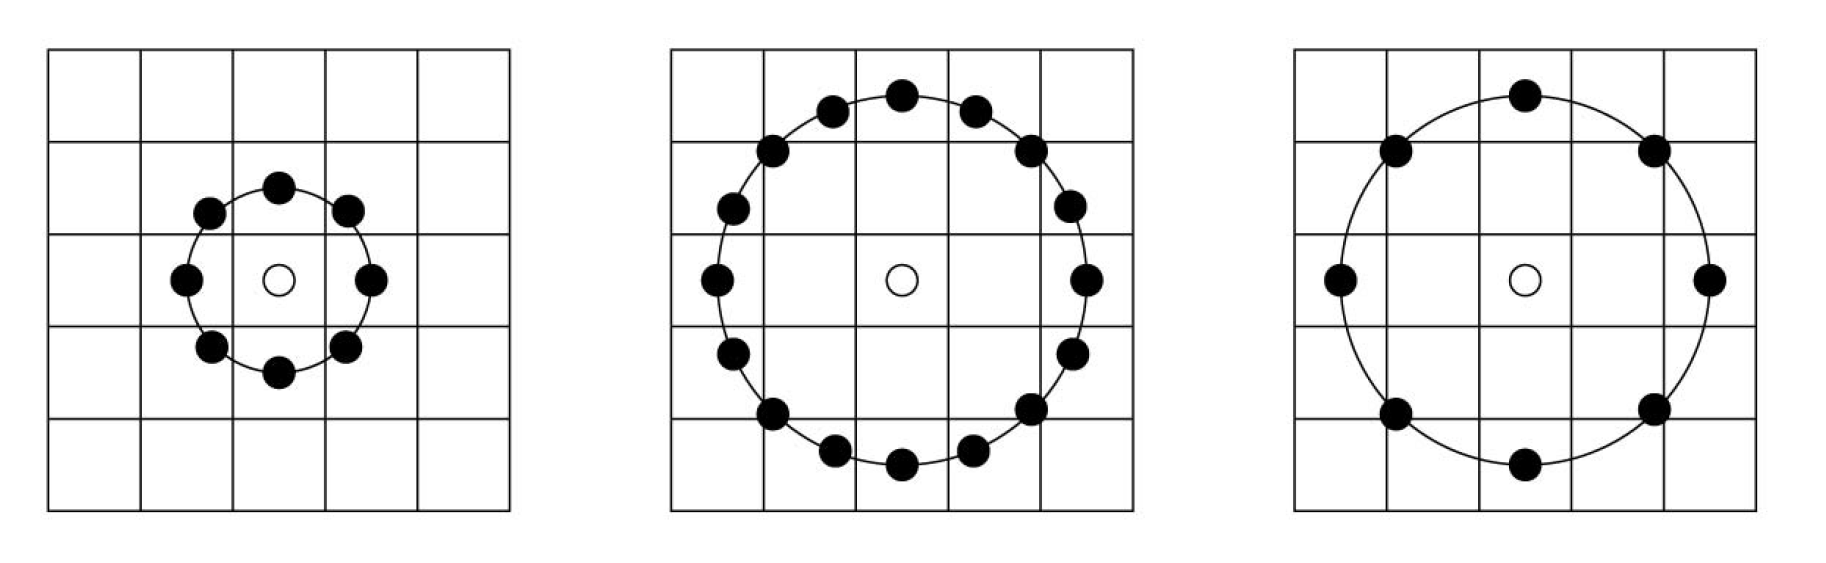
\includegraphics[width=253px]{./img/znazorneni_lbp.png}	
		\caption{Znázornění blocku Převzato z \cite{SrovnaniDeskriptoru}}
\end{figure}

\par Výpočet LBP probíhá podle následujícího vzorce, kde je pixel pro který se hodnoty počítají označen písmenem $c$ (centrální). Algoritmus následně prochází všechny okolní pixely, označené písmenem  $x$. Hodnota daného pixelu je označena jako $p(x)$ a výsledek tohoto porovnání je označen $s(x)$.

\begin{displaymath} 
	\label{asd2} 
		    s(x) = \left\{ \begin{array}{r@{\quad}c}
    		1, & p(x) \geq h(c) \\
    		0, & p(x) < h(c) \\ \end{array} \right. 
\end{displaymath}

\begin{figure}[ht]
	\centering
	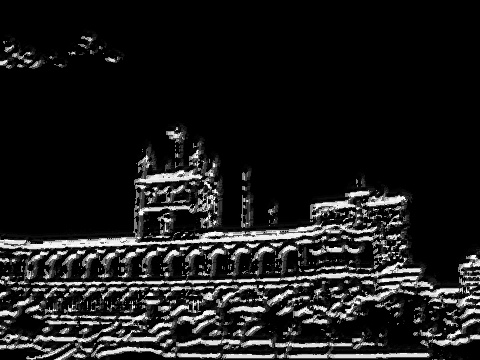
\includegraphics[width=150pt]{./img/lbp1_tau.jpg}
	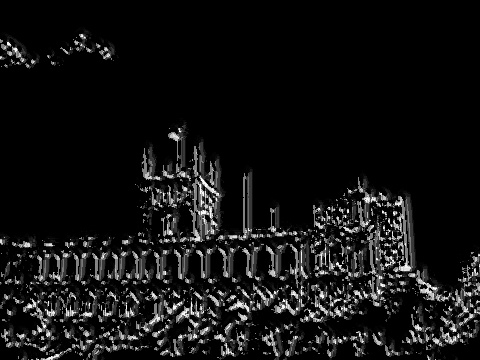
\includegraphics[width=150pt]{./img/lbp2_tau.jpg}
	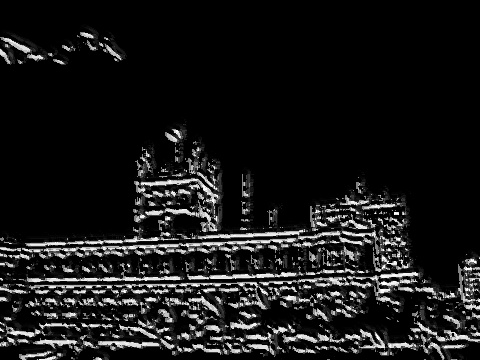
\includegraphics[width=150pt]{./img/lbp3_tau.jpg}
	\caption{Obrázky po aplikaci LBP s použitím $\tau$. Každý obrázek představuje jeden směr.}
\end{figure}

\subsection{Konstrukce globálního histogramu}
\par Obrázky získané z LBP jsou rozdeleny pravidelnou čtvercovou mřížkou. Pro každou vzniklou oblast je vypočten lokální histogram. Vzniklé histogramy jsou zřetězeny. Díky tomu jsou získány tři histogramy pro každý směr jeden, které jsou opět zřetězeny. \\
Rozdělení obrázků a určování lokálních histogramů se dělá za účelem zachování informace o prostorovém rozložení jednotlivých příznaků.

\subsubsection{Uniformní vzory}
Jelikož histogram, který bude vytvořen je velmi dlouhý, je možné ho zkrátit vybíráním pouze tz. uniformních vzorů. Některé binární vzory se totiž na běžných obrázcích vyskytují častěji a to až, dle experimentů z 90 \%. Jsou to právě výše zmíněné uniformní vzory. Uniformní vzory jsou hodnoty čísla (čísla z pohledu binární reprezentace), kdy dochází k maximálně dvěma přechodům z 0 na 1 a nebo opačně. Například 00011110 je uniformní, oproti tomu 01101111 není. Těchto vzorů je 58, všechny ostatní vzory jsou reprezentovány jediným vzorem. Takto je délka jednoho lokálního histogramu zredukována z 256 na 59 binů.

\section{Barevný POEM}
\subsubsection{Výpočet gradientu a magnitudy}
Výpočet gradientu probíhá obdobně jako u nebarevného obrázku. Pro každou ze tří složek jsou získány dvě matice filtrované maskami. Celkem bude $3 \times 2$ matic. Na matice se dá pohlížet jako na 2 vektory o 3 složkách. Vektory jsou sloučeny pomocí součtu vektoru do jednoho 3 složkového vektoru. Magnituda je opět velikost vektoru tentokrát, ale v prostoru. \\
\\
Format vzniklých vektorů 
\begin{align}
	\label{barevny_poem_vznikle_vektory}
			 u = [blue_x, green_x, red_x] \\
			 v = [blue_y, green_y, red_y]
\end{align}

Pomocí součtu vektorů je získán jeden třísložkový vektor:
\begin{align}
   \label{soucet_vektrou} \vec{u} + \vec{v} = (u_1 + v_1, u_2 + v_2, u_3 + v_3 )
\end{align} 

\begin{figure}[H]
    \centering
    \def\svgwidth{\columnwidth}
    \import{img/}{soucet_vektoru.pdf_tex} 
    \caption{Grafické znázornění součtu vektorů. Součet je tvořen z vektorů [4, 8, 10] a [8, 4, 0].}
    %\input{soucet_vektoru.pdf_tex}
\end{figure}

\subsubsection{Diskretizace směru gradientu}
U vektorů získaných v předchozím kroku je určena velikost úhlu mezi vektorem a ekvivalentní vektorem s vynulovanou složkou $z$. Následně je spočítáno do které části kružnice vektor směřuje. Pro znaménkovou reprezentaci je celkový rozsah $0 - \pi$, pro neznaménkovou reprezentaci $0 - 2\pi$.
\\
Při neznaménkové reprezentaci a počtu směrů $d = 3$, jsou následující intervaly $\left(0 - \frac{\pi}{3}\right)$, $\left(\frac{\pi}{3} - \frac{2\pi}{3}\right)$ a  $\left(\frac{2\pi}{3} - \pi\right)$.
\\
Pro výpočet diskretizace směru při neznaménkové reprezentaci je $y$ složka rozdělena na kladnou a zápornou část. To hraje velkou roli, pokud je $y$ složka vektoru záporná. V tom případě je nutné nebrat úhel $\alpha$, ale jeho doplněk ($ 180 - \alpha$).

\begin{figure}[H]
    \centering
    \def\svgwidth{\columnwidth}
    \import{img/}{3D_kruznice.pdf_tex} 
    \caption{Grafické znázorněnní součtu vektorů. Součet je tvořen z vektorů [4, 8, 10] a [8 4, 0].}
    %\input{soucet_vektoru.pdf_tex}
\end{figure}

\subsubsection{Výpočet lokálního histogramu}
U každého směru  se vezmou jednotlivé pixely s jejich okolím a zprůměrují se jejich hodnoty. Toto okolí se nazývá cell. \\

\subsubsection{Zakódování příznaků pomocí LBP}
LBP operátor je aplikován na okolí každého pixelu o velikost $3 \times 3$. Oproti tomu POEM je možné aplikovat na větší okolí. Toto okolí se nazývá block, zpravidla se jedná o kruhové okolí s poloměrem L/2 (L představuje velikost blocku). Pro stanovení intenzit okolních hodnot je možné použít bilineární interpolaci. Pro zvýšení stability v téměř konstantní oblasti lze k centrálnímu pixelu přičítat malou konstantu $\tau$.

\begin{figure}[H]
	\centering
	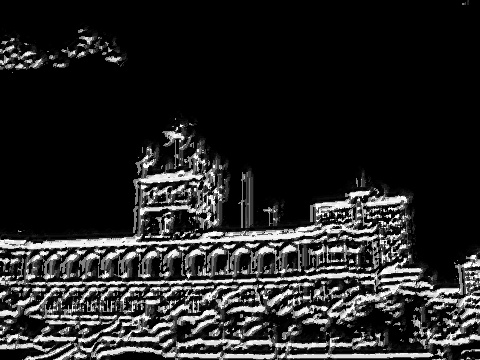
\includegraphics[width=150pt]{./img/lbp_3_1.jpg}
	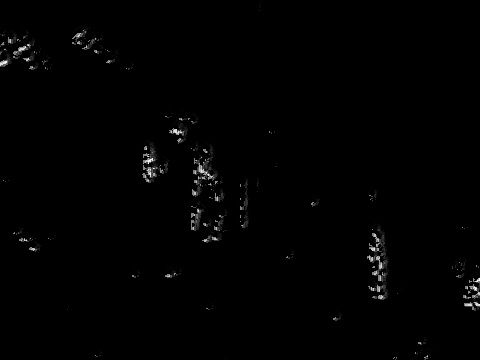
\includegraphics[width=150pt]{./img/lbp_3_2.jpg}
	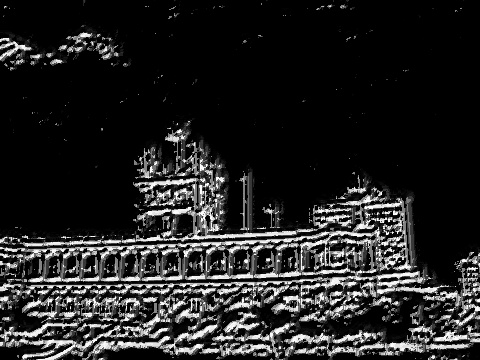
\includegraphics[width=150pt]{./img/lbp_3_3.jpg}
	\caption{Obrázky po aplikaci LBP s použitím $\tau$. Každý obrázek představuje jeden směr.}
\end{figure}

\subsubsection{Konstrukce globálního histogramu}
Obrázky získané z LBP jsou rozdeleny pravidelnou čtvercovou mřížkou. Pro každou vzniklou oblast je vypočten lokální histogram. Vzniklé histogramy jsou zřetězeny. Díky tomu jsou získány tři histogramy pro každý směr jeden, které jsou opět zřetězeny. \\
Rozdělení obrázků a určování lokálních histogramů se dělá za účelem zachování informace o prostorovém rozložení jednotlivých příznaků.

Jelikož histogram, který bude vytvořen je velmi dlouhý, je možné ho zkrátit vybíráním pouze tz. uniformních vzorů. Některé binární vzory se totiž na běžných obrázcích vyskytují častěji a to až, dle experimentů z 90 \%. Jsou to právě výše zmíněné uniformní vzory. Uniformní vzory jsou hodnoty čísla (čísla z pohledu binární reprezentace), kdy dochází k maximálně dvěma přechodům z 0 na 1 a nebo opačně. Například 00011110 je uniformní, oproti tomu 01101111 není. Těchto vzorů je 58, všechny ostatní vzory jsou reprezentovány jediným vzorem. Takto je délka jednoho lokálního histogramu zredukována z 256 na 59 binů.
 

 
\chapter{Přenesení klíčových slov za pomocí práhu}
\par Pro přenesení klíčových slov lze použít algoritmus kdy přeneseme pouze ta klíčová slova, která svými výskyty přesahují předepsaný práh. Je definováno $total\_keywords$ počet všech klíčových slov i s jejich redundantními výskyty, $frequence\_keyword$ jako počet výskytů daného slova v k nejbližších sousedech a $count\_keywords$ jako počet jedinečných klíčových slov (bez redundantních výskytů).  

\par Práh \eqref{prah} je vyčíslen jako jedna děleno (počet všech klíčových slov i s jejich redundantními výskyty - 1). Následuje výpočet váhy pro dané klíčové slovo \eqref{vaha_klicoveho_slova}, které probíhá jako počet výskytů daného slova děleno počet všech klíčových slov i s jejich redundantními výskyty. Pokud je tato hodnota vyšší než práh, je klíčové slovo přeneseno.

\begin{align}
   \label{prah} th = \frac{1}{count\_keywords-1}
\end{align}

\begin{align}
   \label{vaha_klicoveho_slova} vaha = frequence\_keyword / total\_keywords
\end{align}


\chapter{Testovací databáze}
Pro natrénování a následné testování byla použita data z databází IAPRC a ESP. Kolekce obrázků na natrénování musí být pečlivě vybrána aby zahrnovala co možná největši okruh z různých témat. 

\section{iaprtc12}
Sada iaprtc12 je kolekce obrázků přírodních scén která zahrnují různé sporty a akce, fotografie lidí, zvířat, měst, krajin a mnoho jiných aspektů součastného života. Data obsahují \num{20 000} obrázků ve formátu \textit{jpg} s celkovým počtem \num{291} klíčových slov. Ke každému obrázku jsou přiložena metadata ve formátu \textit{XML}, která obsahují informace o obrázku v různých jazycích. Kromě angličtiny je tam i například španělština nebo němčina. V metadatatech ovšem nenajdeme klíčová slova tak jak bychom si je představovali, ale v různých tagách nalezneme například titulek obrázku, který může vypadat například The Plaza de Armas, a v tagu description je například  a woman and a child are walking over the square. Spolu s databází jsme zíkali i klíčová slova která byla z přiložených xml extrahována.\\
K jednomu obrázku je v průměru přiřazeno \num{5.7} klíčových slov. Pro trénovaní bylo použito \num{17 664} obrázků, na následné testování jich bylo použito \num{1960}. 


\begin{figure}[h]
		\centering
		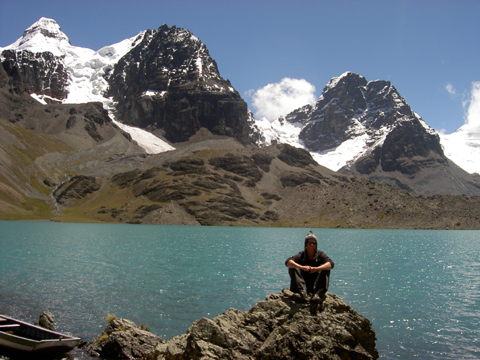
\includegraphics[width=140px]{./img/iaprtc12.jpg}	
		\caption{Ukázka obrázku s klíčovými slovy: front lake man mountain rock sky summit}
\end{figure}

\section{ESP}
\par Sada ESP obsahuje širokou škálů snímku s anotacemi, ze kterých byla použita jen malá část. Konkrétně \num{18 689} obrázků na trénování a \num{2061} na testování. Ke každému obrázku je přiřazen soubor ve formátu \textit{desc}, který obsahuje anglické anotace. Z celkových 269 klíčových slov je k jednomu obrázků přiřazeno v průměru 4.6 slov.

\par Obrázky získaly svá klíčová slova pomocí ESP game, což je hra, která funguje pouze online. V principu spojí dva hráče, kteří nemají možnost spolu komunikovat. Následně je oběma hráčům zobrazen stejný obrázek, který musí popsat co nejvíce různými výrazy v angličtině. V případě, že se hráči shodnou, počítač předpokládá že mu poskytli pravdivou informaci o tom co se na obrázků nachází. Tak si tuto anotaci uloží do databáze a hráči získají body.

\begin{figure}[h]
		\centering
		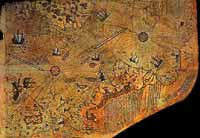
\includegraphics[width=140px]{./img/esp.jpg}	
		\caption{Ukázka obrázku s klíčovými slovy: brown chart country map old orange ship white}
\end{figure}

%Výhodou této sady je, že řeší problém kolektivnýho významu mezi anotátory což vede k anotaci s méně individuální předpojatostí.
%Výhodou této sady je že lidská anotace odráží kolektivní sémantiku dohodu mezi anotátory což vede k anotaci s méně individuální %předpojatostí

\chapter{Návrh systému}
Systém byl navržen jako modulový a to z důvodu snadné obměny některé z častí, což je výhodné zejména pokud bychom potřebovali například spočítat vzdálenosti vektorů podle jiného algoritmu. 

%TODO od Miry: Jak jiˇz bylo zm´ınˇeno v pˇredchoz´ıch kapitol´ach, proces automatick´e anotace
%zahrnuje dva probl´emy – extrakce pˇr´ıznak˚u a samotn´a automatick´a anotace.
%Dalˇs´ım probl´emem je vyhodnocen´ı spr´avnosti v´ysledk˚u. C´ılem n´avrhu architektury
%programu je modul´arnost kaˇzd´eho z probl´emu. Architektura je tedy
%rozdˇelena na tˇri ˇc´asti.Cílem návrhu systému je modulárnost každého problému 
%Strukturu modulu pro pˇredzpracov´an´ı popisuje diagram na obr´azku (9.1).
 

\begin{figure}[ht]
    \centering
    \def\svgwidth{\columnwidth}
    \import{img/}{navrh_systemu.pdf_tex} 
    \caption{Navrh systému.}
    %\input{soucet_vektoru.pdf_tex}
\end{figure}


\chapter{Implementace}
\section{Použité programové prostředky}
\par Program byl navržen na operační systém Linux. Jako programovací jazyk byl zvolen Python a to z důvodu jeho jednoduchého použití, což je na prototyp, jako je tento velice výhodné na časovou náročnost. 

\par Pro spuštění programu je třeba mít nainstalovaný python ve verzi 2.7.12 s NumPy verze 9, knihovnu openCV verzi 3.1 a vědeckou knihovnu scipy verze 0.17.0. Vzhledem k náročnosti programu je pro jeho spuštění nutné mít v počítači alespoň 16 GB RAM paměti a to především z důvodů ukládání mezivýsledků pomocí modulu \textit{pickle}, což je modul pro serializaci objektů. Následující postupy jsou uvedeny pro operační systém Linux, a tak se mohou od postupu na jiném operačním systému lišit.   
  
  
\subsection{OpenCV}
\par OpenCV (Open source computer vision) je knihovna vydávána pod licencí BSD a je volně k dispozici jak pro akademické účely, tak pro komerční použití. Je vhodná pro použití v C++, C, Python a Javě. Podporuje operační systémy Windows, Linux, Mac OS, iOS a Android.

\par Knihovna byla navrhnuta pro výpočetní efektivitu v oblasti počítačového vidění a zpracování obrazu se zaměřením na zpracování obrazu v reálném čase. Z důvodu optimalizace byla napsána v C/C++. 

\par Knihovna OpenCV je dostupná na adrese: http://opencv.org/

\subsection{Scikit}
\par Scikit-image je vědecká knihovna algoritmů pro zpracování obrazu. Je k dispozici zdarma a bez omezení s licencí BSD. Poskytuje dobře zdokumentované API v programovacím jazyce Python a je vyvíjena aktivním mezinárodním týmem spolupracovníků.
\cite{Scikit}

\section{Modulové jednotky programu}
\subsection{Config}
\par Při spuštění programu je nejdříve načten konfigurační soubor, který obsahuje jeho veškerá nastavení. Pro snadné a pohodlné spuštění všech modulů je připraven skript \textit{run.py}. V opačném případě můžeme jednotlivé moduly pouštět postupně.

\vspace{1cm}
Parametry configu:
\begin{itemize}
	\item \textit{TRAIN\_LIST} - Trénovací list obrázků, který by měl obsahovat cesty k obrázkům trénovací sady a jejich klíčová slova ve formátu \textit{cesta\_k\_obrazku; klíčové\_slovo klíčové\_slovo}. Předpokládaný formát \textit{.txt}.
	\item \textit{TEST\_LIST} - Testovací list, který by měl obsahovat cesty k obrázkům testovací sady a jejich klíčová slova ve formátu \textit{cesta\_k\_obrazku; klíčové\_slovo klíčové\_slovo}. Předpokládaný formát \textit{.txt}.
	\item \textit{DATAFILE\_TRAIN} - Soubor do kterého budou uloženy příznakovové vektory, načtenáých obrázků. Předpokládaný formát \textit{.py}.
	\item \textit{PICTURE\_RESULT} - Obrazky a prirazene klicova slova klasifikatorem.
	\item \textit{PICTURE\_TEST\_KEYWORDS} - obrazky s prirazenym slovy od klasifikatoru i s se slovy prirazene clovekem.
	\item \textit{KEYWORDS\_RESULT} - Vysledky klicovych slov, jejich presnost a uplnost.
	\item \textit{COUNT\_NEIGHBORS} - Počet sousedů.
	\item \textit{COUNT\_KEYWORDS} - Počet klíčových slov.
\end{itemize}
Dále jsou v cofingu uvedené jednotlivé metody s očekávanou hodnotou \textit{True} nebo \textit{False} v závyslosti zda se mají použít nebo ne.

\subsection{Load data}
Modul načte obrázky z listů uvedených v configu (\textit{TRAIN\_LIST} a \textit{TEST\_LIST}) a načte příslušné příznaky opět podle configu. Následné jsou celé stuktury listů testovacich nebo trenovacích obrazku uloženy do souboru, opět podle configu \textit{DATAFILE\_TRAIN} popřípadě \textit{DATAFILE\_TEST}.


\subsubsection{Extrakce příznaků}
Jednotlivé výpočty příznaků jsou rozděleneny do zvláštních modulů, aby byla obměna jejich výpočtu snadno nahraditelná. V každém modulu je stěžejní pouze funkce \textit{count\_} a název příslušné metody (např. \textit{count\_haarq}), která je volána právě z modulu load data.


Při počítání barevných histogramů byl zjištěn překvapivý poznatek. V případě kdy je histogram jako datová struktura \textit{list} a až výsledný histogram převeden do \textit{numpy array} je rychlost programu nesrovnatelně větší oproti tomu, když jsou histogramy vytvořeny rovnou jako \textit{numpy array}  
  
\subsection{Knn classifier}
V tomto modulu probíhá počítání vzdáleností mezi jednotlivými příznaky (vektory) a jejich škálování na interval 0 až 1. Z naškálovaných výsledků je spočtena výsledná vzdálenost JEC.    

\subsection{Label transfer}
Modul přenese n nejbližších klíčových slov, podle vzdáleností JEC. Na přenesení máme dva algoritmy. První který byl uvedený u JEC a druhý kdy se přenáší jen klíčová slova která převyšují počtem výskytů práh.   

\subsection{Evaluator}
\par Tento modul vyhodnotí úspěšnosti anotace. Jako prvni získáme všechna klíčová slova a to pomocí funkce \textit{getKeywords}. Pokračujeme získáním anotovaných dat ve funkci \textit{read\_data\_from\_file}.  Následně je pro každé klíčové slovo spočítána přenost a úplnost. Tyto hodnoty jsou popsány v sekci Vyhodnocení výsledků.

\chapter{Vyhodnocení výsledků}
\par Zpracování výsledků probíhá jako porovnání anotací přidělených člověkem s anotacemi přidělenymi klasifikátorem. $w_{auto}$ představuje počet obrázků, kterým bylo dané slovo přiřazeno klasifikátorem, $w_{human}$ počet obrázků, kterým bylo dané slovo přiřazeno člověkem a $w_{corrrectly}$ počet obrázků, kterým bylo slovo přiřazené správně. U klasifikátorů se počítá precision (přesnost) a recall (úplnost) pro každé slovo v testovací sadě. Při testování se snažíme obě hodnoty co nejvíce maximalizovat.

\par Recall \eqref{recall} je počet obrázků správně anotovaných s daným slovem děleno počtem obrázků, kterým bylo toto slovo přiděleno v anotaci člověkem. Precision \eqref{precision} je počet správně anotovaných obrázků s tímto slovem děleno celkovým počtem anotovaných obrázků s tímto slovem (správně nebo ne). 

\begin{align}
   \label{recall} Rec = \frac{w_c}{w_h}
\end{align}
\begin{align}
   \label{precision} Prec = \frac{w_c}{w_a}
\end{align}

\par Výsledná přesnost a úplnost se počítá jako průměr dosažených výsledků pro jednotlivá slova. V případě, že přesnost převyšuje úplnost jsou klíčová slova sice korektní, ale je jich málo. V opačném případě při převyšující úplnosti bylo získáno hodně klíčových slov, ale málo z nich je korektních. Proto je snaha získat obě čísla co nejvyšší. 
\par Počet nenulových slov značí počet slov které byli při anotaci použity alespoň jednou. \cite{Result_A_A}



\section{Srovnání výsledků}
Přesné parametry se kterými autoři dosahovali nejlepší výsledků nebyli zjištěny, proto bylo třeba je u některých příznaků zkoušet metodou pokus omyl.


\subsection{Gabor - porovnání parametrů}
\begin{center}
\begin{tabular}{ |c|c|c|c|c| }
\hline
Parametry & $P_{\%}$ & $R_{\%}$ & N \\ \hline
 lambda $0.25$, $0.5$, $1.0$ & \multirow{3}{*}{9.9} & \multirow{3}{*}{6.8} & \multirow{3}{*}{151} \\
 sigma $1$ & & & \\
 theta $0$, $\frac{\pi}{4}$, $\frac{\pi}{2}$, $\frac{3}{4}\pi$ & & & \\ \hline
 lambda 2, $2\sqrt{2}$, 4 & \multirow{3}{*}{8.5} & \multirow{3}{*}{5.7} & \multirow{3}{*}{143} \\
 sigma $1$ & & & \\
 theta $0$, $\frac{\pi}{4}$, $\frac{\pi}{2}$, $\frac{3}{4}\pi$ & & & \\ 
\hline
\end{tabular}
\captionof{table}{Gábor s knihovnou scikit na datech iaprtc12.}
\end{center}

\subsection{Haar - porovnání parametrům}
\begin{center}
	\begin{tabular}{ |c|c|c|c| }
		\hline
		Parametry & $P_{\%}$  & $R_{\%}$ & N \\ \hline
		Desktiptor jako vektor $12 \times 16$ binů & 2.9 & 2.1 & 63 \\ \hline
		Deskriptor jako vektor sum & 5.8 & 4 & 114 \\ \hline 	
	\end{tabular}
	\captionof{table}{Haar na datech iaprtc12.}
\end{center}

\subsection{Přiřazování klíčových slov pomocí práhu}
\begin{center}
\begin{tabular}{l | c c c|c c c}
		          	& \multicolumn{3}{c|}{5 sousedů} & \multicolumn{3}{ c}{10 sousedů} \\ 
Metoda          		& $P_{\%}$ & $R_{\%}$ & N & $P_{\%}$ & $R_{\%}$ & N \\
\hline
RGB						& 20.1 & 9 & 178 & 14.3 & 15.3 & 205 \\
LAB					  	& 17.1 & 8.8 & 156 & 14.4 & 14.7 & 185 \\
HSV            			& 21 & 11.4 & 191 & 14.9 & 18.6 & 221 \\
RGB, LAB, HSV      		& 21.9 & 11.2 & 188 & 16.1 & 19 & 221 \\
\hline
\hline
JEC						& 0 & 0 & 0 & 0 & 0 & 0 \\ 
\end{tabular}
\captionof{table}{Výsledky získané přiřazování klíčových slov s práhem na datech iaprtc12. P značí přesnost, R úplnost a N počet nenulových klíčových slov.}
\end{center}

\subsection{Konečné výsledky a srovnání s literaturou}
\begin{center}
\begin{tabular}{l | c c c|c c c}
		          	& \multicolumn{3}{c|}{IAPRTC12} & \multicolumn{3}{ c}{ESP} \\ 
Metoda          		& $P_{\%}$ & $R_{\%}$ & N & $P_{\%}$ & $R_{\%}$ & N \\
\hline
RGB						& 14.1 & 9 & 167 & 17 & 13.2 & 209 \\
LAB					  	& 12.7 & 7.5 & 148 & 6.1 & 5.2 & 117 \\
HSV            			& 16.7 & 10.9 & 181 & 18.2 & 14.8 & 211 \\
RGB, LAB, HSV      		& 17.4 & 11.1 & 178 & 18.7 & 14.8 & 209 \\
Gabor					& 8.1 & 4.7 & 126 & 14.2 & 10.8 & 194 \\
GaborQ					& 6.9 & 4.8 & 133 & 12.1 & 9.9 & 187 \\
Haar					& 5.8 & 4 & 114 & 10.2 & 8.4 & 178 \\
HaarQ					& 5.8 & 4.4 & 123 & 9.4 & 7.3 & 169 \\
POEM		     		& 21.5 & 12.8 & 189 & 0 & 0 & 0 \\
RGB, LAB, HSV, POEM		& 21.8 & 13.8 & 187 & 3.3 & 3.3 & 85  \\
Barevný POEM			& 21 & 12.4 & 184 & 0 & 0 & 0 \\
\hline
\hline
JEC						& 0 & 0 & 0 & 0 & 0 & 0 \\ 
\end{tabular}
\captionof{table}{Výsledky získané v rámci práce. P značí přesnost, R úplnost a N počet nenulových klíčových slov.}
\end{center}

\begin{center}
	\begin{tabular}{l | c c c|c c c}
		          	& \multicolumn{3}{ c|}{IAPRTC12} & \multicolumn{3}{ c }{ESP} \\ 
	Metoda          		& $P_{\%}$ & $R_{\%}$ & N & $P_{\%}$ & $R_{\%}$ & N  \\
	\hline
	RGB						& 20 & 13 & 189 & 21 & 17 & 221 \\
	LAB					  	& 22 & 14 & 194 & 20 & 17 & 221 \\
	HSV            			& 18 & 12 & 190 & 18 & 15 & 217  \\
	Haar					& 17 & 8 & 161 & 21 & 14 & 210  \\
	HaarQ					& 16 & 10 & 173 & 19 & 14 & 210 \\
	Gabor					& 14 & 9 & 169 & 16 & 12 & 199 \\
	GaborQ					& 8 & 6 & 137 & 14 & 11 & 205 \\
	\hline
	\hline
	JEC						& 25 & 16 & 196 & 23 & 19 & 227 \\ 
	\end{tabular}
	\captionof{table}{Výsledky z literatury \cite{JEC2}.}
\end{center}
\chapter{Závěr}
\par V práci byla řešena automatická anotace obrázků pomocí spojování barevných a texturových příznaků. U prvního řešení s metodou JEC byla použito vypočtení příznaků odděleně následováno spojení jejich vzdáleností do jedné.  V druhém případě bylo spojení příznaků interpretováno jako jeden společný příznak, kdy byl POEM rozšířen na všechny barevné kanály.
\par V teoretické části byly popsány a rozebrány nízkoúrovňové příznaky barva a textura. U barvy se zabývalo barevnými modely RGB, LAB a HSV. U textury to byl GABOR, HAAR a POEM. Dála se zabývalo přenášení klíčových slov za pomocí práhu, kdy musela frekvence výskytu u sousedů převýšit stanovený práh. 
\par V praktické byl navržen a implementován program v jazyce python pro automatickou anotaci obrázků, který využívá právě vyše zmíněné barevné prostory a reprezentace textur. Na základě naměřených výsledků byly laděny optimální parametry. V rámci práce byla prostudovaná a použita knihovna openCV. Funkčnost programu byla otestována na databázích iaprtc12 a ESP.
\par Vylepšení programu barevného poemu. 

 
 
% 
% PRO ANGLICKOU SAZBU JE NUTNÉ ZMĚNIT
% CITAČNÍ STYL!
%

\chapter{Použité zkratky}


\begin{labeling}{zkratky}
	\item [AIA] Automatic image anotation.	
	\item [JEC] Joint equal contribution
	\item [RGB] Barevný model Red, Green, Blue (červená, zelená, modrá).
	\item [LAB] Barevný model. 
	\item [HSV] Barevný model. 
	\item [POEM] Patterns of oriented edge magnitudes.
	\item [LBP] Local binary pattern.
	\item [OpenCV] Open source computer vision.
	\item [BSD] Licence pro svobodný software, umožňující volné šíření softwaru.
\end{labeling}

\bibliographystyle{csplainnatkiv}
{\raggedright\small
\bibliography{literatura}
}

\appendix
\chapter{Uživatelská dokumentace}
\par Pro spuštění programu je třeba mít nainstalovaný python ve verzi 2.7.12 s NumPy verze 9, knihovnu openCV verzi 3.1 a vědeckou knihovnu scipy verze 0.17.0. Vzhledem k náročnosti programu je pro jeho spuštění nutné mít v počítači alespoň 16 GB RAM paměti. Následující postupy jsou uvedeny pro operační systém Linux, které se od postupu na jiném oparečním systému mohou lišit.

\par Veškeré nastavení aplikace probíhá pomocí souboru \textit{config.py}

\vspace{1cm} 
Parametry configu:
\begin{itemize}
	\item \textit{TRAIN\_LIST} - Trénovací list obrázků, který by měl obsahovat cesty k obrázkům trénovací sady a jejich klíčová slova ve formátu \textit{cesta\_k\_obrazku; klíčové\_slovo klíčové\_slovo}. Předpokládaný formát \textit{.txt}.
	\item \textit{TEST\_LIST} - Testovací list, který by měl obsahovat cesty k obrázkům testovací sady a jejich klíčová slova ve formátu \textit{cesta\_k\_obrazku; klíčové\_slovo klíčové\_slovo}. Předpokládaný formát \textit{.txt}.
	\item \textit{DATAFILE\_TRAIN} - Soubor do kterého budou uloženy příznakovové vektory, načtenáých obrázků. Předpokládaný formát \textit{.py}.
	\item \textit{PICTURE\_RESULT} - Obrazky a prirazene klicova slova klasifikatorem.
	\item \textit{PICTURE\_TEST\_KEYWORDS} - obrazky s prirazenym slovy od klasifikatoru i s se slovy prirazene clovekem
	\item \textit{KEYWORDS\_RESULT} - Vysledky klicovych slov, jejich presnost a uplnost
	\item \textit{COUNT\_NEIGHBORS} - Počet sousedů.
	\item \textit{COUNT\_KEYWORDS} - Počet klíčových slov.
\end{itemize}
Dále jsou v cofingu uvedené jednotlivé metody s očekávanou hodnotou \textit{True} nebo \textit{False} v závyslosti zda se mají použít nebo ne.

\subsubsection{Spuštění programu}
Program spustíme z příkazové řádky zadáním příkazu \textit{python nazevskriptu.py}. 
\begin{itemize}
	\item \textit{python run.py} - v případě spuštění všech skriptů postupně.
	\item \textit{python load\_data.py} - v případě načtení dat, získání příznaků z načtených obrázků a následné uložení do souboru uvedeného v configu.
	\item \textit{python count\_distance\_jec.py} - spočítání vzdáleností a přiřadí klíčová slova.
	\item \textit{python count\_count\_result.py} -vyhodnotí úspěšnost klasifikace mimo jiné přesnost a úplnost.
\end{itemize}

\subsubsection{Výstupy programu}
Názvy výstupných souborů se mohou lišit v závyslosti na nastavení configu.
\begin{itemize}
	\item \textit{PICTURE\_RESULT} - Obrazky a prirazene klicova slova klasifikatorem.
	\item \textit{PICTURE\_TEST\_KEYWORDS} - obrazky s prirazenym slovy od klasifikatoru i s se slovy prirazene clovekem
	\item \textit{KEYWORDS\_RESULT} - Vysledky klicovych slov, jejich presnost a uplnost
	\item \textit{DATAFILE\_TRAIN} - Soubor do kterého budou uloženy příznakovové vektory, načtenáých obrázků. 
\end{itemize}
	
\end{document}
